% Created with jtex v.1.0.20
\documentclass{article}
\usepackage{hyperref}
\usepackage{datetime}
\usepackage{graphicx}
\usepackage{natbib}
\bibliographystyle{abbrvnat}

%%%%%%%%%%%%%%%%%%%%%%%%%%%%%%%%%%%%%%%%%%%%%%%%%%
%%%%%%%%%%%%%%%%%%%%  imports  %%%%%%%%%%%%%%%%%%%
\usepackage{booktabs}
%%%%%%%%%%%%%%%%%%%%%%%%%%%%%%%%%%%%%%%%%%%%%%%%%%


% colors for hyperlinks
\hypersetup{colorlinks=true, allcolors=blue}

\newcommand{\logo}{
  \href{https://curvenote.com}{
\includegraphics[width=2cm]{curvenote.png}}
}

\title{Map Descriptive Analysis}

\author{Sunghyun Ahn \and Megan Dhillon \and Yoohan Park \and Breitling Snyder}

\newdate{articleDate}{18}{12}{2025}
\date{\displaydate{articleDate}}

\begin{document}
\maketitle
\begin{center}\logo\end{center}


\begin{verbatim}

\end{verbatim}

\begin{verbatim}
import geopandas as gpd
import pandas as pd
import matplotlib.pyplot as plt
import matplotlib.patches as mpatches
import os

out_dir = "visualizations/descriptive_maps"
os.makedirs(out_dir, exist_ok=True)

import sys
sys.path.append("..")
from CEStools.utils import clean_data, qmap
\end{verbatim}

\begin{verbatim}
shp_path = "../data/calenviroscreen40_shp/CES4 Final Shapefile.shp"
shape = gpd.read_file(shp_path)
\end{verbatim}

\begin{verbatim}
shape = clean_data(shape, keep_geom=True)
shape = shape.to_crs(epsg=3857)
\end{verbatim}

\begin{verbatim}
shape.head()
\end{verbatim}

\bigskip\noindent
\begin{tabular}{p{\dimexpr 0.045\linewidth-2\tabcolsep}p{\dimexpr 0.045\linewidth-2\tabcolsep}p{\dimexpr 0.045\linewidth-2\tabcolsep}p{\dimexpr 0.045\linewidth-2\tabcolsep}p{\dimexpr 0.045\linewidth-2\tabcolsep}p{\dimexpr 0.045\linewidth-2\tabcolsep}p{\dimexpr 0.045\linewidth-2\tabcolsep}p{\dimexpr 0.045\linewidth-2\tabcolsep}p{\dimexpr 0.045\linewidth-2\tabcolsep}p{\dimexpr 0.045\linewidth-2\tabcolsep}p{\dimexpr 0.045\linewidth-2\tabcolsep}p{\dimexpr 0.045\linewidth-2\tabcolsep}p{\dimexpr 0.045\linewidth-2\tabcolsep}p{\dimexpr 0.045\linewidth-2\tabcolsep}p{\dimexpr 0.045\linewidth-2\tabcolsep}p{\dimexpr 0.045\linewidth-2\tabcolsep}p{\dimexpr 0.045\linewidth-2\tabcolsep}p{\dimexpr 0.045\linewidth-2\tabcolsep}p{\dimexpr 0.045\linewidth-2\tabcolsep}p{\dimexpr 0.045\linewidth-2\tabcolsep}p{\dimexpr 0.045\linewidth-2\tabcolsep}p{\dimexpr 0.045\linewidth-2\tabcolsep}}
\toprule
 & CIscoreP & OzoneP & PM2\_5\_P & DieselPM\_P & PesticideP & Tox\_Rel\_P & TrafficP & DrinkWatP & Lead\_P & CleanupP & ... & UnemplP & HousBurdP & PopCharP & Hispanic & White & AfricanAm & NativeAm & OtherMult & AAPI & geometry \\
\hline
0 & 69.162885 & 10.566273 & 10.031114 & 52.408214 & 92.034483 & 9.914979 & 63.4000 & 11.165230 & 36.118463 & 17.077268 & ... & 18.310776 & 69.150824 & 79.828543 & 68.9210 & 20.8899 & 0.4004 & 0.2670 & 1.3126 & 8.2091 & POLYGON ((-13406867.885 4155533.339, -13404832... \\
\hline
1 & 70.637922 & 11.561917 & 10.454263 & 39.365277 & 99.586207 & 10.265066 & 19.9000 & 52.828775 & 43.805923 & 72.396417 & ... & 69.130661 & 60.101394 & 56.555724 & 78.6229 & 13.2240 & 2.5051 & 0.0000 & 0.9489 & 4.6990 & POLYGON ((-13406867.885 4155533.339, -13406867... \\
\hline
2 & 61.069087 & 10.566273 & 9.931549 & 60.311139 & 93.827586 & 10.515129 & 42.7500 & 11.165230 & 75.072464 & 2.071669 & ... & 35.020822 & 53.624842 & 67.183560 & 65.7214 & 30.6088 & 0.9591 & 0.0000 & 2.1685 & 0.5421 & POLYGON ((-13404824.281 4156507.571, -13404832... \\
\hline
3 & 5.988401 & 13.615432 & 10.653391 & 34.275047 & 95.413793 & 7.864466 & 39.9250 & 32.559011 & 11.077505 & 0.000000 & ... & 58.355023 & 16.311787 & 10.741301 & 22.9537 & 69.1948 & 0.9342 & 0.7117 & 2.5356 & 3.6699 & POLYGON ((-13403841.327 4147463.306, -13403732... \\
\hline
4 & 23.121533 & 13.615432 & 10.690728 & 18.481643 & 63.241379 & 7.714429 & 24.3625 & 32.559011 & 49.514808 & 2.071669 & ... & 92.399792 & 12.002535 & 46.280888 & 33.4082 & 59.7804 & 0.6986 & 1.4721 & 1.3723 & 3.2685 & POLYGON ((-13406428.948 4147489.901, -13404941... \\
\hline
\bottomrule
\end{tabular}

\bigskip

5 rows $\times$ 31 columns

\begin{verbatim}
burden = "CIscoreP"
\end{verbatim}

\begin{verbatim}
exposure_vars = ["OzoneP", "PM2_5_P", "DieselPM_P", "TrafficP", "Tox_Rel_P", "PesticideP"]
shape["ExposureIdx"] = shape[exposure_vars].mean(axis=1, skipna=True)
\end{verbatim}

\begin{verbatim}
race_cols = ['Hispanic','White','AfricanAm','NativeAm','OtherMult','AAPI']
race_bins = [5, 10, 20, 40, 60, 80, 100]
for race in race_cols:
    print(f" - - - {race} - - -")

    # 1: Map depicting race share (for each race)
    qmap(
        shape,
        race,
        title=f"{race} share (fixed bins)",
        cmap="plasma",
        bins=race_bins,
        save=f"../visualizations/descriptive_maps/race_{race}_fixedbins.png"
    )

    # 2) Bivariate map: race share (x) vs burden (y), 3 \times3 quantiles

    df = shape[[race, burden, "geometry"]].dropna().copy()

    # quantile bins: 0 = low, 1 = mid, 2 = high
    df["race_bin"] = pd.qcut(df[race], 3, labels=False, duplicates="drop")
    df["burden_bin"] = pd.qcut(df[burden], 3, labels=False, duplicates="drop")

    df["bi"] = df["race_bin"].astype(int) + 3 * df["burden_bin"].astype(int)

    # rows = burden (low to high), cols = race (low to high)
    colors = [
        "#e8e8e8", "#b5c0da", "#6c83b5",   # low burden
        "#b8d6be", "#90b2b3", "#567994",   # mid burden
        "#73ae80", "#5a9178", "#2a5a5b"    # high burden
    ]
    df["color"] = df["bi"].map(lambda i: colors[int(i)])

    fig, ax = plt.subplots(1, 1, figsize=(10,10))
    ax.set_axis_off()

    # base map
    shape.plot(ax=ax, color="lightgrey", edgecolor="white", linewidth=0.05)
    df.plot(ax=ax, color=df["color"], edgecolor="white", linewidth=0.05)

    ax.set_title(
        f"Bivariate: {race} share ( \rightarrow) vs {burden} (↑), 3 \times3 quantiles",
        fontsize=14
    )

    # legend (3 \times3 grid)
    leg = fig.add_axes([0.67, 0.12, 0.22, 0.22])
    leg.set_xticks([]); leg.set_yticks([]); leg.set_frame_on(True)

    k = 0
    for j in range(3):          # burden: low -> high
        for i in range(3):      # race: low -> high
            leg.add_patch(
                plt.Rectangle((i, j), 1, 1, facecolor=colors[k], edgecolor="none")
            )
            k += 1

    leg.set_xlim(0, 3); leg.set_ylim(0, 3)
    leg.set_xlabel(f"{race} \rightarrow", fontsize=9)
    leg.set_ylabel(f"{burden} \rightarrow", fontsize=9)
    plt.savefig(
        f"../visualizations/descriptive_maps/bivariate_{race}_{burden}.png",
        dpi=300,
        bbox_inches="tight"
    )
    plt.show()

    # 3) Overlap hotspots: top 10% burden AND top 20% race share
    cut_hi = shape[race].quantile(0.80)
    burden_hot = shape[burden].quantile(0.90)
    overlap = (shape[burden] >= burden_hot) & (shape[race] >= cut_hi)

    fig, ax = plt.subplots(1, 1, figsize=(10,10))
    ax.set_axis_off()
    shape.plot(ax=ax, color="lightgrey", edgecolor="white", linewidth=0.05)
    shape.loc[overlap].plot(ax=ax, color="crimson", edgecolor="white", linewidth=0.05)
    ax.set_title(f"Overlap hotspots: top 10% {burden} AND top 20% {race} share", fontsize=14)
    plt.savefig(
        f"../visualizations/descriptive_maps/overlap_hotspots_{race}_{burden}.png",
        dpi=300,
        bbox_inches="tight"
    )
    plt.show()
\end{verbatim}

\begin{verbatim}
- - - Hispanic - - -
\end{verbatim}

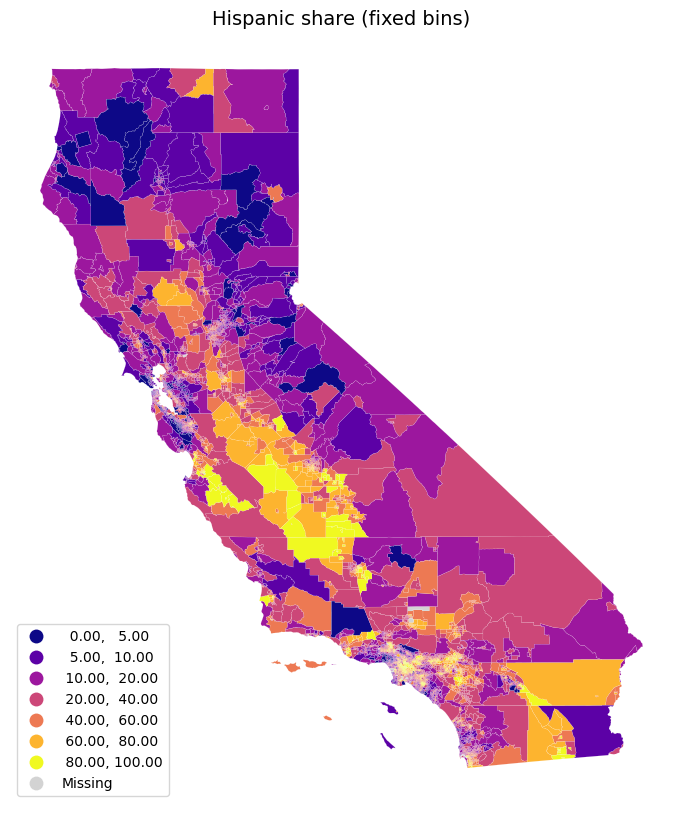
\includegraphics[width=0.7\linewidth]{files/834bcacb264a8121e85becda1d57d517.png}

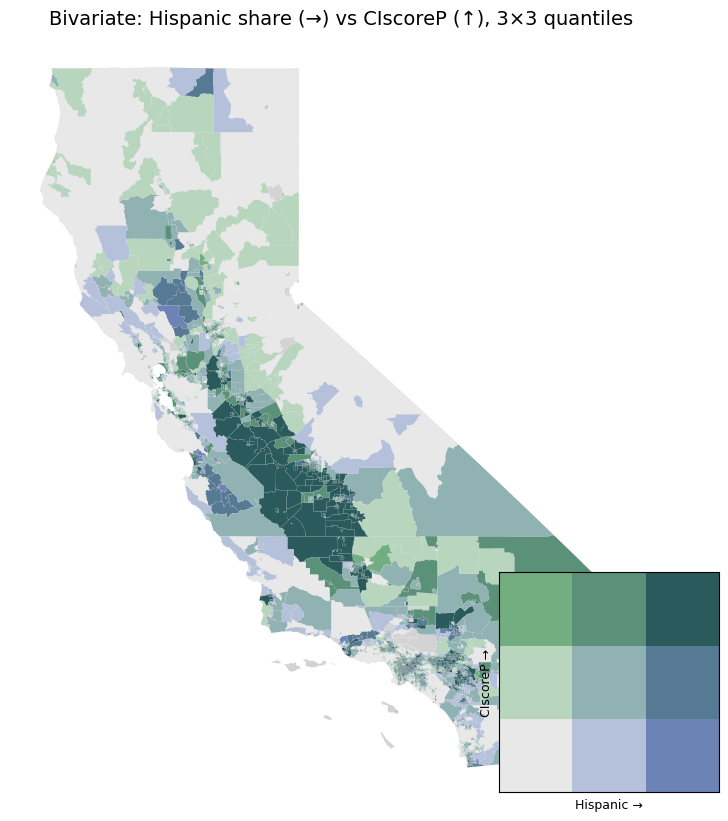
\includegraphics[width=0.7\linewidth]{files/e3893b484cf8319cc1514f68fdb50c45.png}

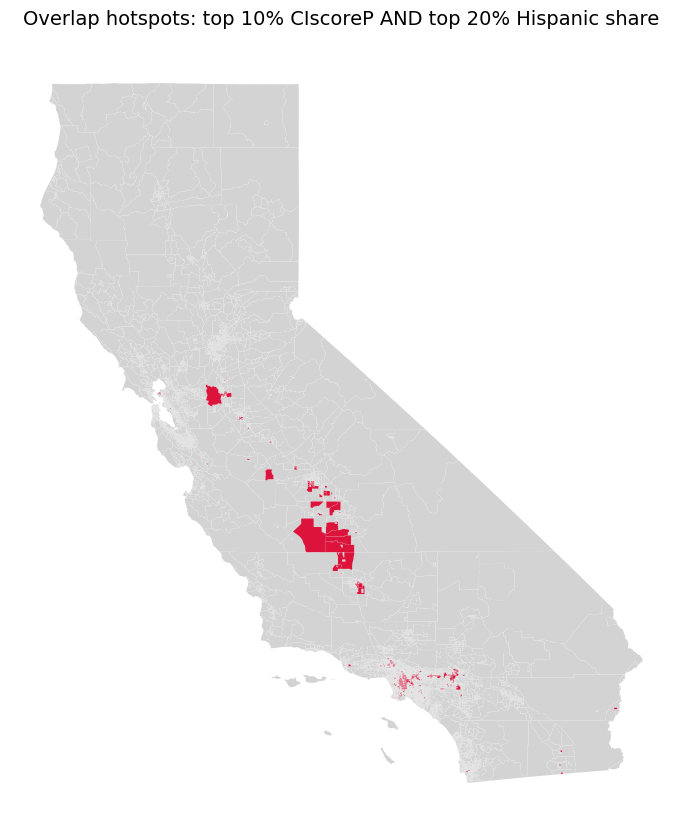
\includegraphics[width=0.7\linewidth]{files/4282a6c5973a8023cffb09624d218ad4.png}

\begin{verbatim}
- - - White - - -
\end{verbatim}

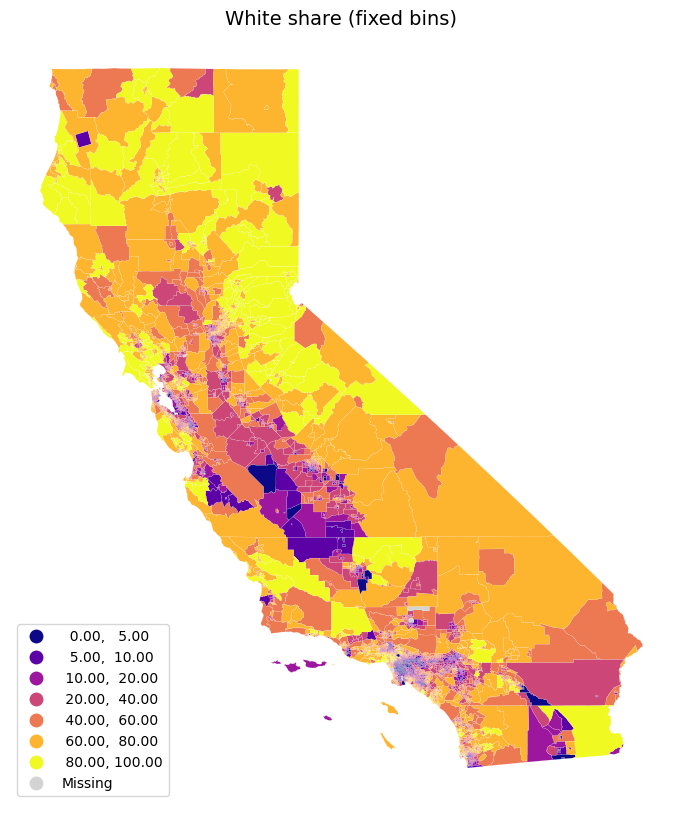
\includegraphics[width=0.7\linewidth]{files/bbe7ecb48912b2a0eeadde1b0192be15.png}

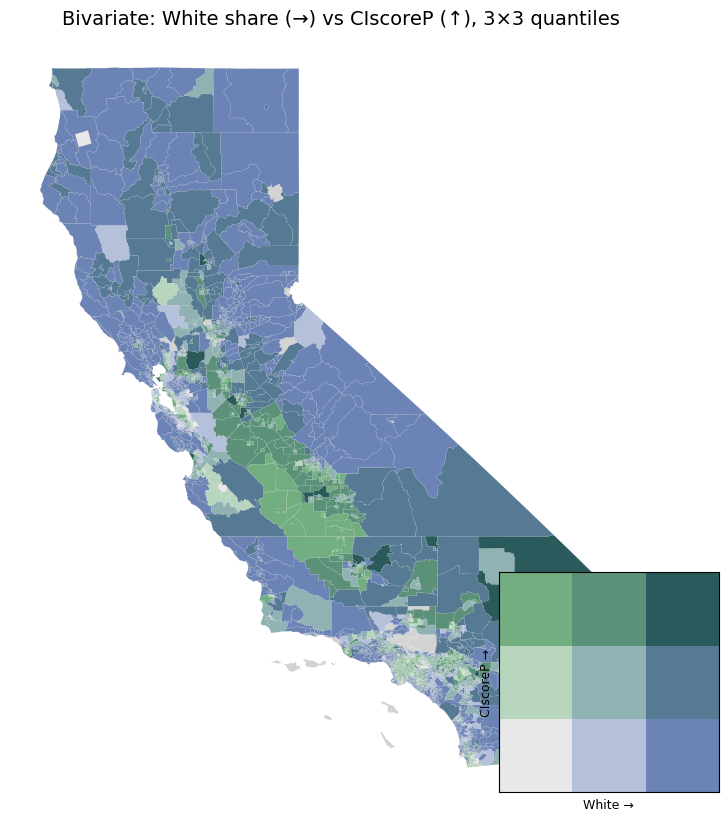
\includegraphics[width=0.7\linewidth]{files/b462b2f86511a8a2daec0b49d39a4e19.png}

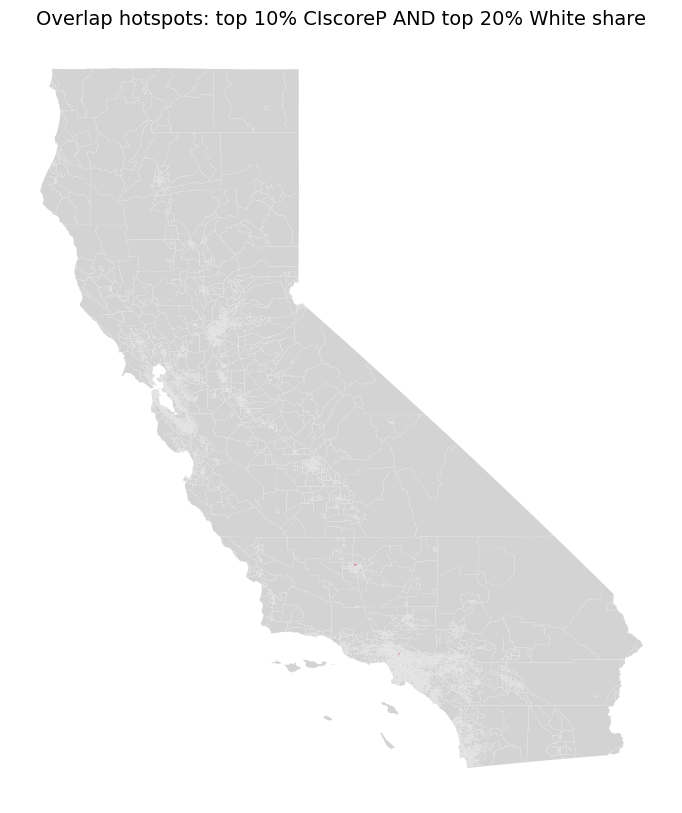
\includegraphics[width=0.7\linewidth]{files/9b37ebb424f57dd23bdbb0d4377a8c70.png}

\begin{verbatim}
- - - AfricanAm - - -
\end{verbatim}

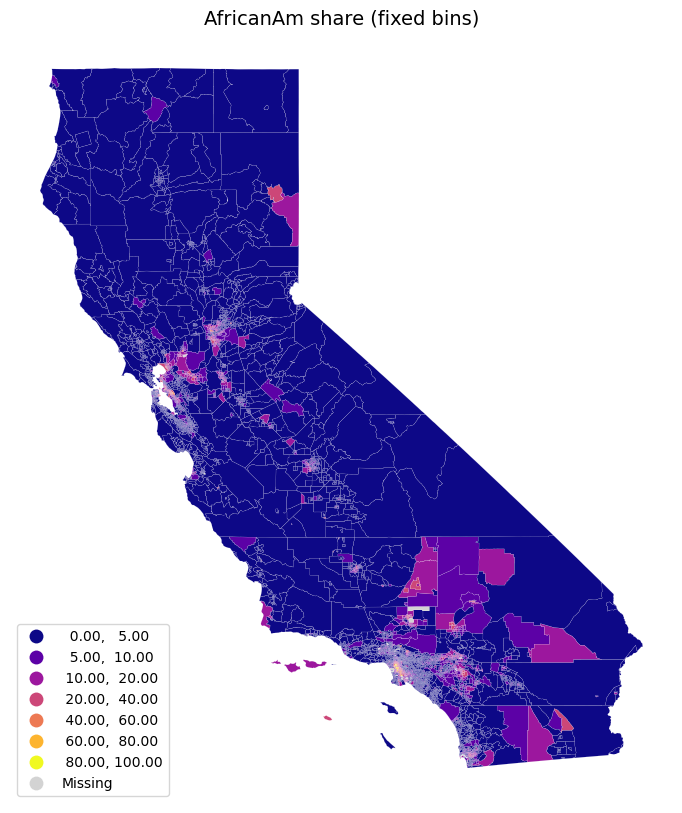
\includegraphics[width=0.7\linewidth]{files/d368f763a6fa8fa192ea51b9f2c67a91.png}

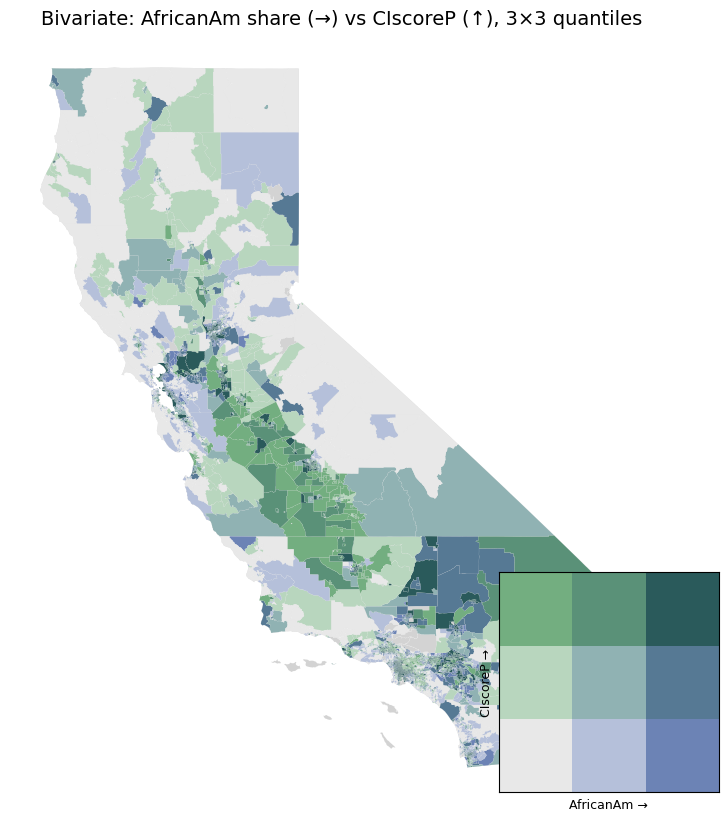
\includegraphics[width=0.7\linewidth]{files/e40e5a08997f0954feaed37f6f1ec810.png}

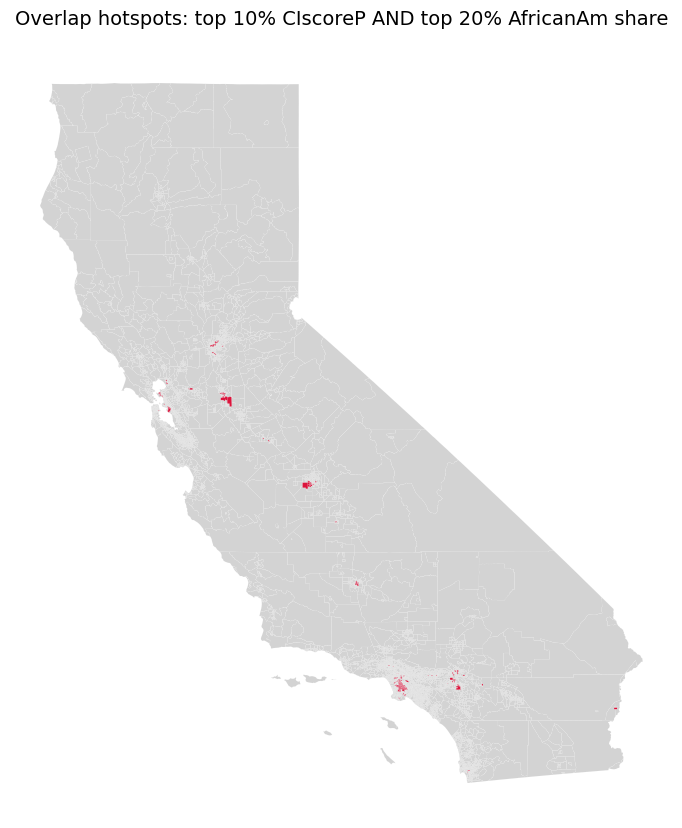
\includegraphics[width=0.7\linewidth]{files/f8256e7d831e041f4eb4c62da94af75e.png}

\begin{verbatim}
- - - NativeAm - - -
\end{verbatim}

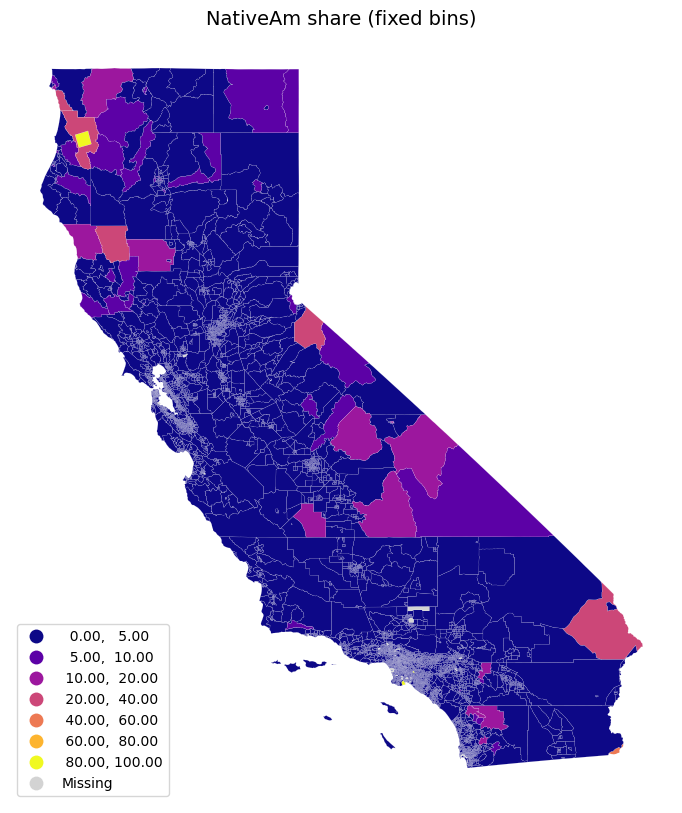
\includegraphics[width=0.7\linewidth]{files/cf47f64b8315b32f39c0a0836e609c90.png}

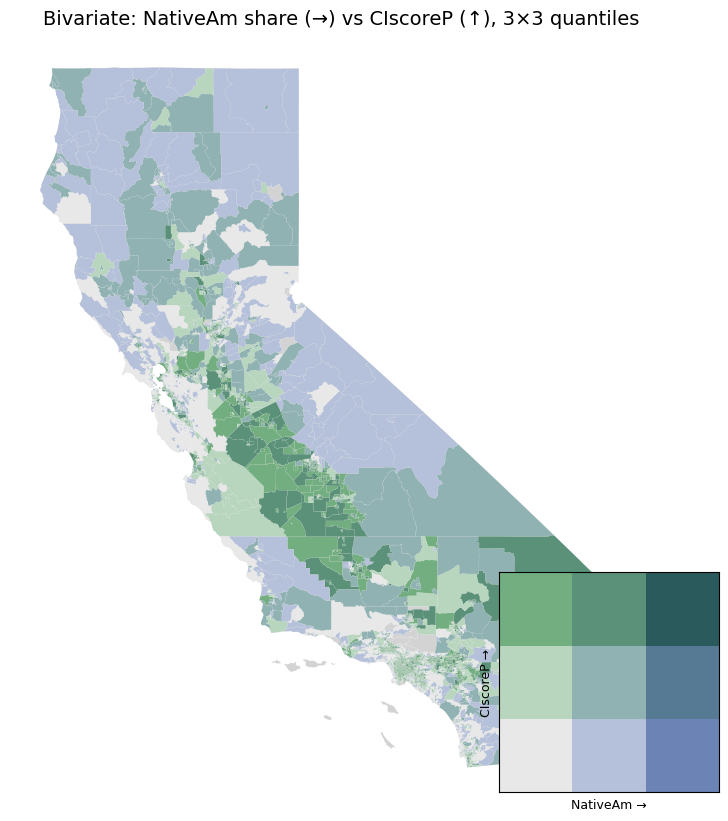
\includegraphics[width=0.7\linewidth]{files/6785d8f65566feddf34e122956db1ea4.png}

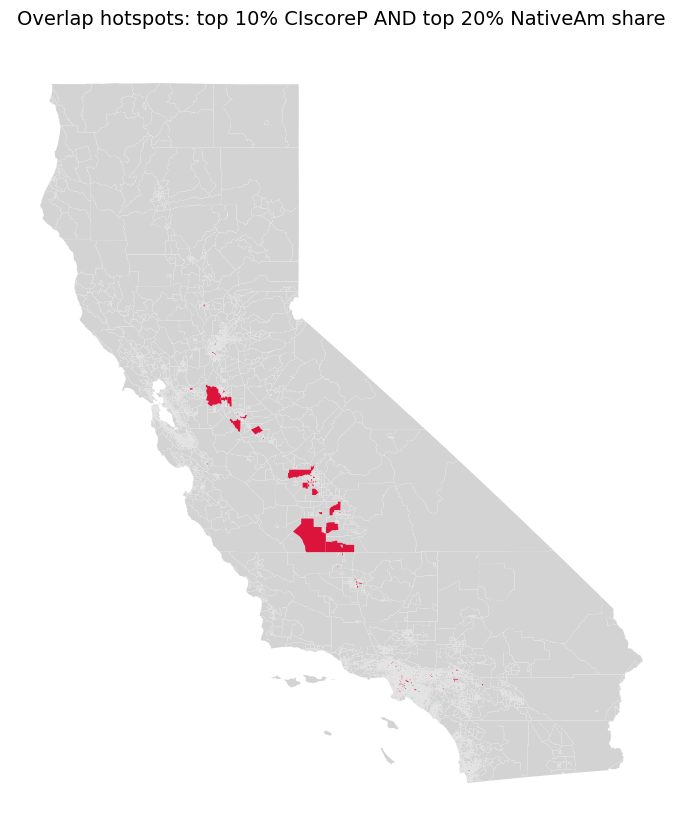
\includegraphics[width=0.7\linewidth]{files/3e988d80fa3ab738a53c82f5c2d6ef1a.png}

\begin{verbatim}
- - - OtherMult - - -
\end{verbatim}

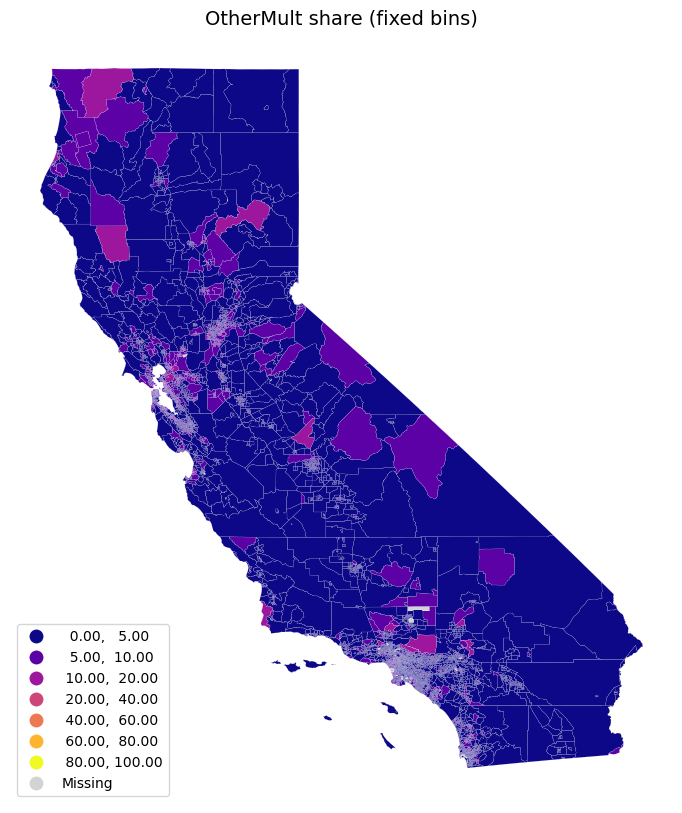
\includegraphics[width=0.7\linewidth]{files/2ed911e02666131413f79d5e7a026249.png}

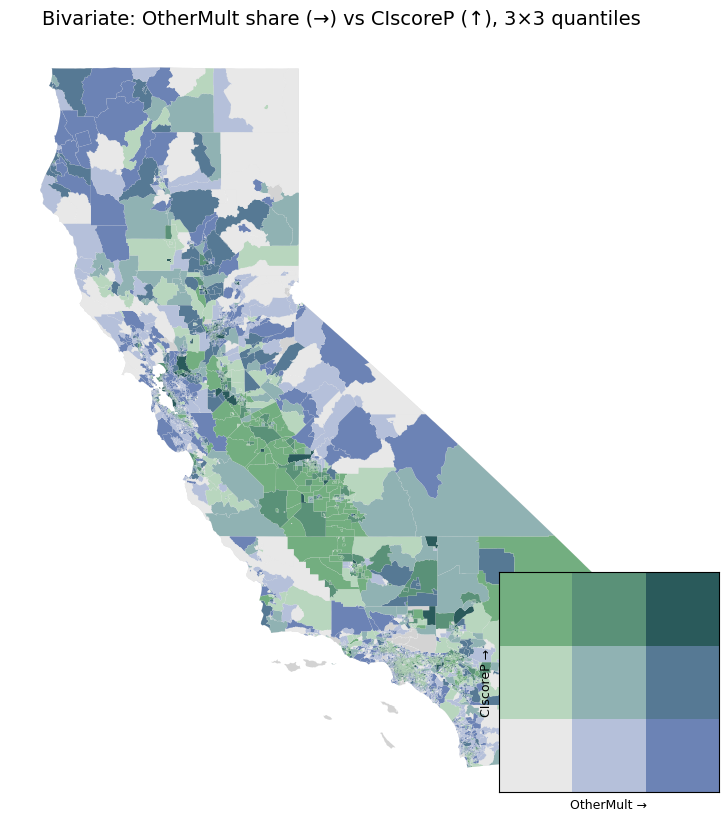
\includegraphics[width=0.7\linewidth]{files/9b7102d403057d47c42e5f60ccfb9887.png}

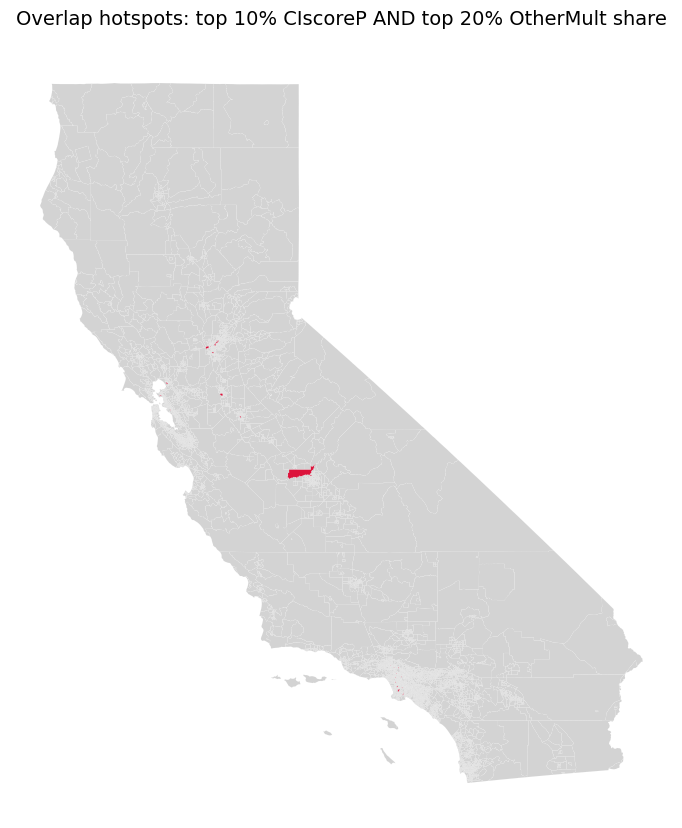
\includegraphics[width=0.7\linewidth]{files/fc7ba5247ec180d7bc01e4baa0ad611e.png}

\begin{verbatim}
- - - AAPI - - -
\end{verbatim}

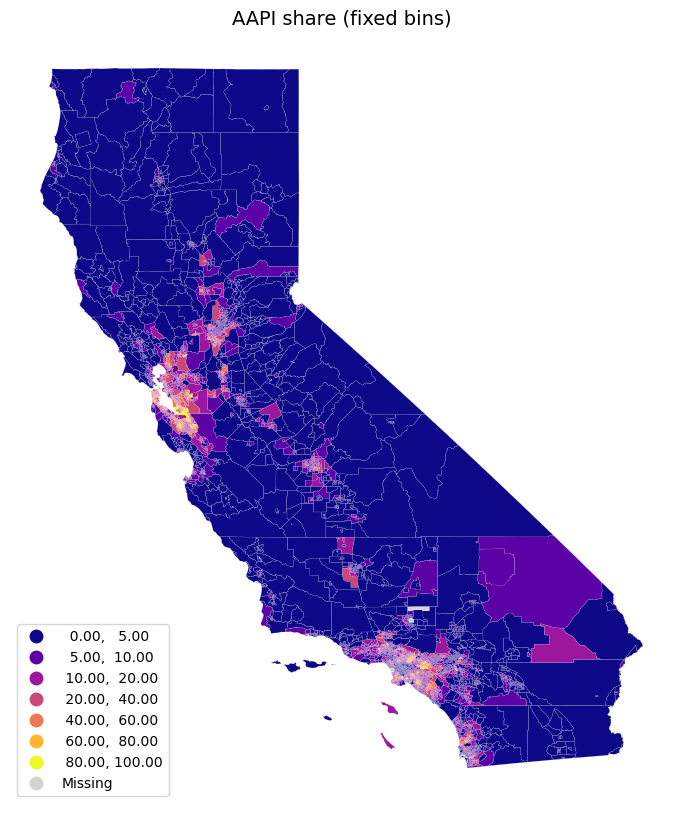
\includegraphics[width=0.7\linewidth]{files/e6aab51b6528376ea00df55957d38b36.png}

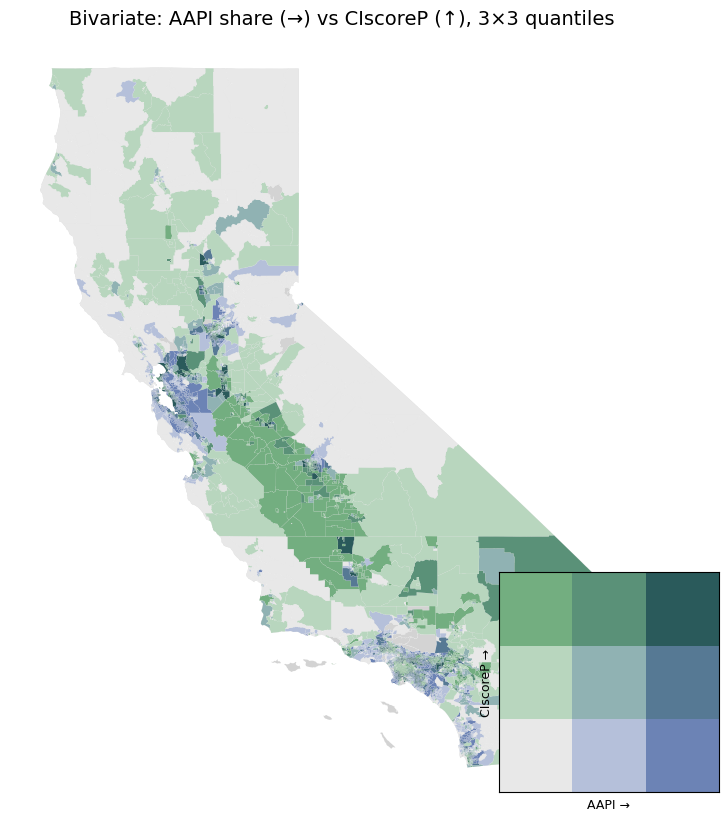
\includegraphics[width=0.7\linewidth]{files/ffc211b13fa9ef3bb12479ca6a0d5b9e.png}

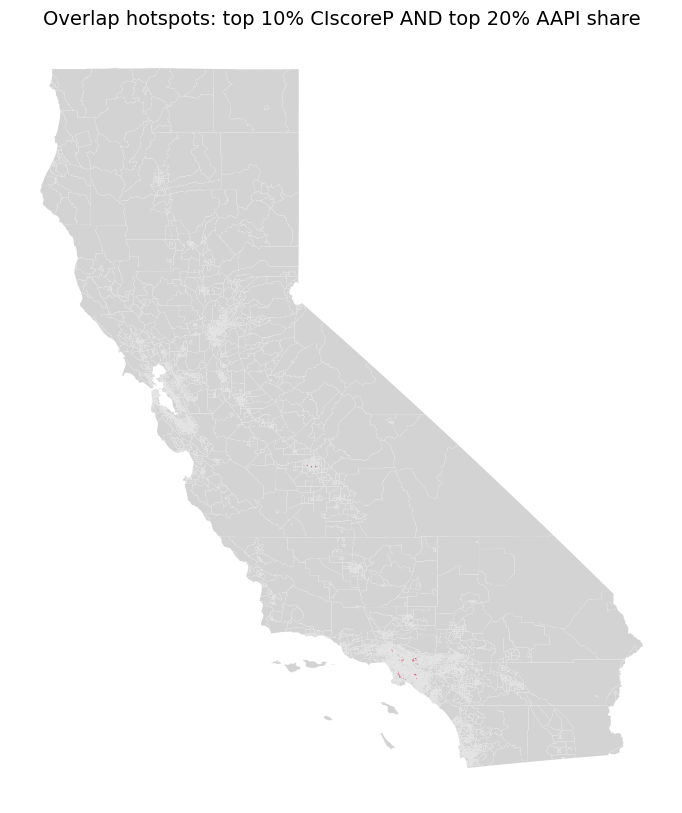
\includegraphics[width=0.7\linewidth]{files/c6150cc02512e873f7a4c2713f8357e9.png}


\end{document}
